
    \chapter{Referencial teórico}
    
    \section{Segurança da informação}
    Segurança da informação é o conjunto de práticas, políticas, procedimentos e tecnologias que tem como objetivo proteger as informações de uma organização. A segurança de uma determinada informação pode ser afetada por fatores comportamentais e de uso de quem se utiliza dela, pelo ambiente ou infraestrutura que a cerca ou por pessoas mal intencionadas que têm o objetivo de furtar, destruir ou modificar tal informação.
    
    Para implementar aplicações seguras, \citeonline{Hintzbergen2018} descreve que é necessário implementar um conjunto adequado de controles, políticas, processos, procedimentos, estruturas e funções tanto de software, quanto de hardware. Existe a necessidade de estabelecer, implementar, monitorar, revisar e melhorar onde necessário, para ter certeza que os objetivos específicos da segurança da informação estão sendo atendidos. Esse objetivo é manter os pilares principais da segurança da informação, que são a confidencialidade, integridade, disponibilidade e, mesmo não citados em todas as literaturas, autenticidade e não-repúdio.
    
    \subsection{Confidencialidade}
    A confidencialidade, segundo \citeonline{Machado2014}, se refere a capacidade de garantir que o nível necessário de sigilo seja aplicado em cada junção de dados em processamento. Além disso, trata-se dos limites em termos de quem pode obter que tipo de informação, isso é, o ato de garantir que a informação seja acessível apenas àqueles autorizados a ter acesso. Nomes, CPFs, números de cartão, transações e registros financeiros, entre outras informações sensíveis, devem ter acesso autorizado somente aos indivíduos com permissão para ver tal informação. 
    
    Ela garante que o nível necessário de sigilo seja aplicado em cada elemento de processamento de dados e impede a divulgação não autorizada. Esse nível de confidencialidade deve prevalecer enquanto os dados residirem em sistemas e dispositivos na rede, quando forem transmitidos e quando chegarem ao seu destino.
    
    Este pilar pode ser fornecida através da criptografia de dados à medida que são armazenados e transmitidos, usando preenchimento de tráfego na rede, estrito controle de acesso, classificação dos dados e treinamento de pessoal nos procedimentos apropriados.
    
    \subsection{Integridade}
    A integridade, segundo \citeonline{Machado2014}, é a garantia de rigor e confiabilidade das informações de um sistema e de que não ocorrerão modificações não autorizadas de dados. Uma informação uma vez armazenada, espera-se que ela se mantenha integra, isso é, correta, autêntica e confiável. 
    
    Os dados devem ser protegidos contra exclusão e modificação por parte não autorizada, enquanto estão em uso, em trânsito e quando são armazenados, independentemente de residirem em um laptop, dispositivo de armazenamento, data center ou na nuvem. Mesmo que um indivíduo autorizado fizer alterações por engano, essas alterações devem poder ser revertidas.
    
    \subsection{Disponibilidade}
    A disponibilidade, segundo \citeonline{Machado2014}, refere-se capacidade que os sistemas e as redes devem ter para executar e disponibilizar sempre que necessários, mesmo diante de eventos adversos, os dados de forma previsível e adequada às necessidades. Eles devem estar aptos a recuperar quedas de disponibilidade de forma rápida e segura e a garantir que a produtividade das operações do provedor não seja afetada significativamente. 
    
    Para manter a disponibilidade, as organizações implementam estratégias de redundância, backups regulares e planos de continuidade de negócios. Essas medidas são cruciais em ambientes nos quais a interrupção dos serviços pode resultar em prejuízos substanciais, como no setor financeiro ou em serviços de emergência. A disponibilidade não apenas implica a prevenção de falhas, mas também a rápida recuperação diante de situações imprevistas, garantindo a continuidade operacional.
    
    \subsection{Autenticidade}
    A autenticidade, segundo \citeonline{Hintzbergen2018}, foca na verificação da identidade de usuários, sistemas ou dados. Em transações digitais, a autenticidade é essencial para prevenir acessos não autorizados e estabelecer a confiança nas comunicações. Métodos como senhas, PIN, autenticação de dois fatores e biometria são implementados para garantir que apenas entidades legítimas tenham acesso aos recursos. 
    
    A autenticidade é particularmente crítica em setores nos quais a validação da identidade é fundamental, como em sistemas de pagamento online ou em ambientes corporativos que exigem controle de acesso rigoroso.
    
    \subsection{Não-repúdio}
    O princípio de não repúdio, segundo \citeonline{Hintzbergen2018}, visa garantir que o autor não negue ter criado e assinado o documento. Ele é vital para garantir que as partes envolvidas em uma transação digital não possam negar sua autoria ou participação. Este pilar é alcançado por meio do uso de assinaturas digitais, registros de auditoria e outros mecanismos que geram evidências irrefutáveis das ações realizadas. 
    
    Nos setores legais e financeiros, o não repúdio é essencial para a validação de transações, pagamentos e contratos, garantindo a responsabilidade das partes envolvidas nos processos. Este princípio não apenas reforça a confiabilidade nas interações digitais, mas também contribui para a solução de disputas e questões de conformidade.
    
    \section{Sistema operacional Android}
    O Android \cite{Doc2024} é um sistema operacional de código aberto baseado no kernel Linux, desenvolvido inicialmente pela Android Inc. e adquirido pelo Google em 2005. Lançado oficialmente em 2008, o Android rapidamente se tornou o sistema operacional móvel dominante no mercado global, sendo utilizado por uma ampla variedade de dispositivos, incluindo smartphones, tablets, smartwatches, televisões e automóveis. A arquitetura do Android é composta por várias camadas, como mostrado na figura \ref{android}, cada uma desempenhando um papel crucial na funcionalidade e segurança do sistema. Essas camadas incluem o kernel do Linux, responsável pela comunicação entre o hardware e o software, gerenciamento de recursos, segurança e drivers de dispositivo; bibliotecas nativas escritas em C/C++ que fornecem suporte para várias funcionalidades, como gráficos, bancos de dados e multimídia; Android Runtime, o runtime que executa aplicações Android e substituiu o Dalvik Virtual Machine, proporcionando melhor desempenho e menor consumo de memória; framework de aplicações, um conjunto de APIs que permite aos desenvolvedores criar aplicações, fornecendo acesso a serviços do sistema como gerenciador de atividades, gerenciador de janelas e provedores de conteúdo; e as aplicações do sistema, que são aplicativos pré-instalados que fornecem funcionalidades básicas como telefone, e-mail, navegador web e contatos.
    
    \begin{figure}[H]
    \centering 
    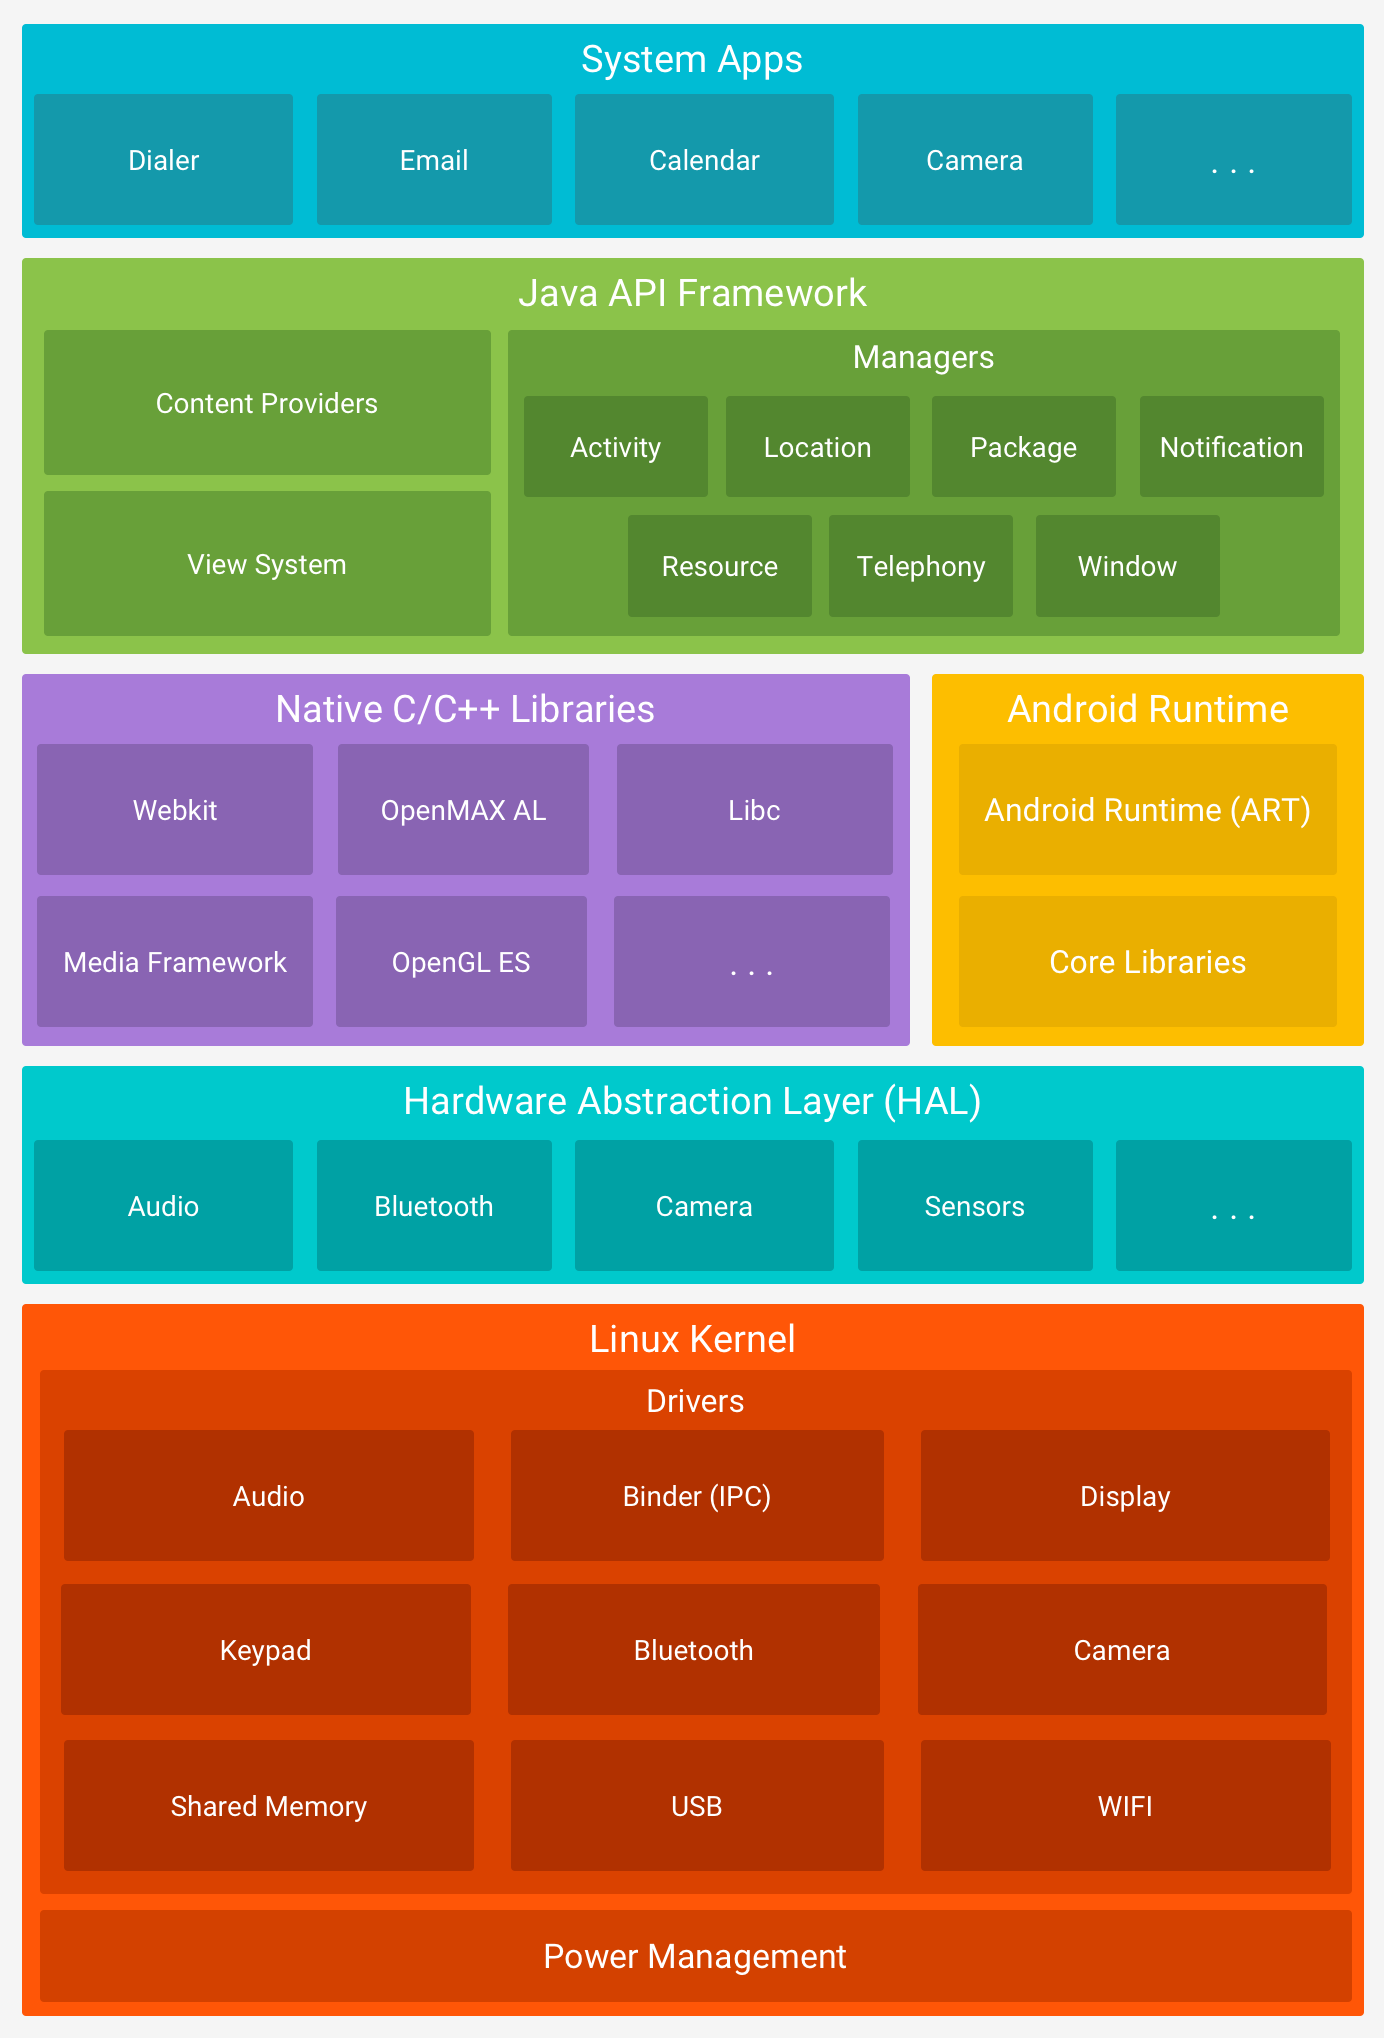
\includegraphics[width=12cm]{Imagens/arqandroid.png} 
    \caption{Arquitetura do Android}
    \label{android}
    \cite{Doc2024}
    \end{figure}

    
    \subsection{Componentes do android}
    Segundo \citeonline{Elenkov2014}, os aplicativos Android são uma combinação de componentes fracamente acoplados e com vários pontos de acesso. Cada componente pode oferecer vários pontos de entrada que podem ser alcançados com base nas ações do usuário no mesmo ou em outro aplicativo, ou acionados por um evento do sistema sobre o qual o aplicativo registrou para ser notificado.

    Os componentes são definidos no arquivo manifesto do aplicativo, chamado AndroidManifest.xml, que é um arquivo que descreve informações essenciais sobre a aplicação para as ferramentas de build do Android, para o sistema operacional Android e para o Google Play. 
    
    Os componentes principais e descritos por \citeonline{Elenkov2014} são:

    \subsubsection{Activities}
    Uma activity é uma tela única com uma interface de usuário. Elas são os principais blocos de construção dos aplicativos da GUI do Android. Um aplicativo pode ter várias atividades e, embora geralmente sejam projetadas para serem exibidas em uma ordem específica, cada atividade pode ser iniciada de forma independente, potencialmente por um aplicativo diferente (se permitido).
    
    \subsubsection{Services}
    Um service é um componente executado em segundo plano e não tem interface de usuário. Esses componentes são normalmente usados para executar alguma operação de longa duração, como baixar um arquivo ou reproduzir música, sem bloquear a interface de usuário. Eles também podem definir uma interface remota e fornecer alguma funcionalidade para outros aplicativos. No entanto, diferentemente dos serviços do sistema, que fazem parte do sistema operacional e estão sempre em execução, os serviços do aplicativo são iniciados e interrompidos sob demanda.
    
    \subsubsection{Content providers}
    Os content providers fornecem uma interface para dados do aplicativo, que normalmente são armazenados em um banco de dados ou arquivos. Eles podem ser acessados via comunicação entre processos e são usados principalmente para compartilhar os dados de um aplicativo com outros aplicativos. Os content providers oferecem controle refinado sobre quais partes dos dados são acessíveis, permitindo que um aplicativo compartilhe apenas um subconjunto de seus dados.
    
    \subsubsection{Broadcast receivers}
    Um broadcast receivers é um componente que responde a eventos de todo o sistema, chamados transmissões. As transmissões podem se originar do sistema (por exemplo, anunciando alterações na conectividade de rede) ou de um aplicativo de usuário (por exemplo, anunciando que a atualização de dados em segundo plano foi concluída).
    
    \subsection{Mecanismos de segurança do sistema operacional}
    \label{mecanismos}
    De acordo com \citeonline{Doc2024}, o Android incorpora diversos mecanismos de segurança destinados a proteger o sistema e os dados do usuário contra ameaças e ataques. \citeonline{Stevenson2021} descreve alguns deles: 

    \subsubsection{Sandboxing}
    O Android atribui automaticamente um identificador de usuário único, frequentemente chamado de ID de aplicativo, a cada aplicação no momento da instalação e executa essa aplicação em um processo dedicado rodando com aquele identificador. Assim, as aplicações são isoladas ou colocadas em sandbox, isso é, um ambiente de computação controlado que permite a realização de ações de forma privativa, sem riscos, interferências e modificações externas; tanto no nível do processo quanto no nível de arquivos. 
    
    \subsubsection{Permissões}
    Como as aplicações Android são isoladas em sandboxs, elas só podem acessar seus próprios arquivos e quaisquer recursos do dispositivo que sejam acessíveis a todos. Contudo, uma aplicação com tais restrições não seria muito interessante. Para permitir uma funcionalidade mais rica, o Android pode conceder direitos de acesso adicionais e mais detalhados às aplicações. Esses direitos de acesso são chamados de permissões.

    De maneira simples, uma permissão é simplesmente uma string que denota a capacidade de executar uma operação específica. A operação de destino pode ser coisas desde acessar um recurso físico ou dados compartilhados até a capacidade de iniciar ou acessar um componente em um aplicativo de terceiros. Definir parâmetros como  \textbf{protectionLevel} = ``signature'' (permite apenas aplicações assinadas da mesma forma de acessar o componente) e  \textbf{permission} = ``android .permission.READ\_PROVIDER'' (permite apenas a leitura de informações do componente), são algumas formas de exigir permissões para acessar componentes de uma aplicação
    
    \subsubsection{IPC}
    A comunicação entre processos ou Inter-Process Communication (IPC) no Android é um aspecto crucial do desenvolvimento de aplicações, permitindo que componentes de diferentes aplicações ou de diferentes partes de uma mesma aplicação possam interagir de maneira segura e eficiente. O Android oferece várias ferramentas e mecanismos para facilitar essa comunicação; como Intents e exportação de componentes. Os mecanismos de IPC do Android permitem conferir a identidade do aplicativo que está se conectando à sua IPC e definir políticas de segurança para cada mecanismo.

    \subsubsubsection{Intent}
    Uma Intent é uma descrição abstrata de uma operação a ser realizada. Ela pode ser usada para iniciar um Activity, solicitar informação a um Content Provider ou para se comunicar com um Service. Elas fornecem recursos para executar vinculação tardia de tempo de execução entre o código em diferentes aplicativos. Seu uso mais significativo é no lançamento de atividades, onde pode ser pensado como a cola entre as atividades. É basicamente uma estrutura de dados passiva que contém uma descrição abstrata de uma ação a ser executada.

    \subsubsubsection{Componentes exportados}]
    O Android desenvolveu um parâmetro chamado \textbf{exported}, que define se um componente pode ser iniciado por componentes de outros aplicativos ou não:

    Se \textbf{True}, qualquer aplicativo pode acessar a atividade e iniciá-la pelo nome exato da classe.
    
    Se \textbf{False}, somente componentes do mesmo aplicativo, aplicativos com o mesmo ID de usuário ou componentes de sistema privilegiados podem realizar ações.

    \subsubsection{Desafios de segurança}
    Segundo \citeonline{Hermans2023}, apesar desses robustos mecanismos de segurança, o Android enfrenta vários desafios devido à sua natureza aberta e à fragmentação do ecossistema. A diversidade de dispositivos e versões do Android pode dificultar a distribuição uniforme de atualizações de segurança, deixando alguns dispositivos vulneráveis por longos períodos. A abertura do ecossistema permite que desenvolvedores distribuam aplicações fora da Google Play Store, aumentando o risco de instalação de aplicativos maliciosos. Ademais, os fabricantes de dispositivos podem modificar o Android, potencialmente introduzindo novas vulnerabilidades ou dificultando a aplicação de patches de segurança padrão. Além dos desafios sistêmicos, as vulnerabilidades a nível de aplicação, citadas na seção \ref{owasp}, também representam uma ameaça significativa à segurança no Android. 
    
    \section{Vulnerabilidades, ameaças, riscos e exposição}
    \citeonline{Garg2023} classificam vulnerabilidades como defeitos de segurança suscetíveis a exploração, podendo comprometer os pilares da segurança de um sistema. Estas fragilidades podem se manifestar em diferentes camadas, desde falhas de software até configurações inadequadas e podem ser utilizadas para crimes cibernéticos, para violar a sua privacidade, perturbar a infraestrutura e criar riscos para a segurança nacional. Identificar, corrigir, evitar e principalmente conhecer essas vulnerabilidades é crucial para mitigar riscos e garantir que sistemas permaneçam resilientes diante de potenciais ameaças.
    
    \subsection{OWASP Mobile Top 10 2023 e ciberataques}
    \label{owasp}
    
    O OWASP Mobile Top 10, vista na tabela \ref{tab:owasptt}, é uma lista das principais ameaças e vulnerabilidades de segurança encontradas em aplicações móveis. É um guia elaborado pela organização Open Web Application Security Project (\citeonline{owasp2023}) e uma referência crucial para desenvolvedores, arquitetos de segurança, avaliadores de segurança e quaisquer profissional envolvido com segurança ou desenvolvimento de aplicações mobile. 

    \begin{table}[H]
    \centering
    \caption{OWASP Mobile Top 10 2024}
    \label{tab:owasptt}
    \begin{tabular}{|l|}
    \hline
    \rowcolor[HTML]{68CBD0} 
    \multicolumn{1}{|c|}{\cellcolor[HTML]{68CBD0}{\color[HTML]{FFFFFF} \textbf{OWASP Mobile Top 10 2024: Final Release Updates}}} \\ \hline
    M1: Uso impróprio de credenciais                                                                                              \\ \hline
    M2: Segurança inadequada da cadeia de suprimentos                                                                             \\ \hline
    M3: Autenticação/Autorização Insegura                                                                                         \\ \hline
    M4: Validação de entrada/saída insuficiente                                                                                   \\ \hline
    M5: Comunicação Insegura                                                                                                      \\ \hline
    M6: Controles de privacidade inadequados                                                                                      \\ \hline
    M7: Proteções binárias insuficientes                                                                                          \\ \hline
    M8: Configuração incorreta de segurança                                                                                       \\ \hline
    M9: Armazenamento de dados inseguro                                                                                           \\ \hline
    M10: Criptografia insuficiente                                                                                                \\ \hline
    \end{tabular}
    \end{table}
    
    
    A lista, citada acima, identifica e descreve as vulnerabilidades mais comuns e críticas que são encontradas e exploradas em aplicativos móveis, abrangendo desde questões de autenticação e autorização até problemas relacionados à criptografia e gestão de sessões. O OWASP Mobile Top 10 não apenas destaca os desafios de segurança enfrentados pelas aplicações móveis, mas também orienta a comunidade de desenvolvimento na adoção de boas práticas e na implementação de métodos de segurança eficazes contra estas vulnerabilidades. O guia é atualizado frequentemente, tendo como ultima atualização a de 2023, para acompanhar as mudanças no cenário de ameaças, garantindo que os profissionais estejam sempre atualizados e equipados para enfrentar os desafios emergentes na segurança de aplicações móveis. Segundo a própria organização, as vulnerabilidades são descritas em \cite{owasp2023}.
    
     
    \section{Aplicações Bancárias}
    \label{bancos}
    
    Os serviços bancários móveis compartilham as necessidades críticas de segurança da informação de outros aplicativos, mas diferem em alguns aspectos de implementação e preocupações específicas \cite{Ahmad2015}.
    
    \subsection{Desafios, ameaças e remediações}
    
    Todos os tipos de sistemas são alvos de criminosos cibernéticos. Por conta disso, muitas ameaças diferentes são encontradas e mecanismos de segurança são adotados para garantir a segurança dos sistemas.

    Dessa forma foi realizada uma revisão na literatura com o objetivo de encontrar as mais críticas ameaças e vulnerabilidades encontradas nas aplicações bancárias e suas respectivas remediações e soluções. Resultando nas informações compiladas na seguinte tabela \ref{tab:vuln}: 
    

    \begin{table}[H]
    \centering
    \caption{Principais vulnerabilidades em aplicações bancárias}
    \label{tab:vuln}
    \begin{tabular}{|p{5cm}|p{5cm}|p{5cm}|}
    \hline
    \textbf{Referência} & \textbf{Vulnerabilidades e Ameaças} & \textbf{Soluções e Remediações} \\ \hline
    
    \citeonline{Chen2020} & Vulnerabilidades relacionadas a criptografia imprópria, autenticação inválida e armazenamento inseguro. & Proposta de AUSERA para identificar vulnerabilidades; boas práticas em criptografia e autenticação. \\ \hline
    
    \citeonline{Yildirim20219} & Falhas de dispositivo (permissões, armazenamento de dados e senhas fracas), Rede (MITM e problemas de criptografia) e Data Center (injeção de código). & Uso correto de criptografia, certificados digitais, autenticação multifator (2FA), gerenciamento de sessões e CAPTCHA. \\ \hline
    
    \citeonline{Darem2023} & Phishing, malware, DDoS, ataques man-in-the-middle, ataques de senha e computação quântica. & Criptografia de dados em repouso e em trânsito, segmentação de rede, firewalls, IPS, autenticação multifator, e políticas legais e organizacionais. \\ \hline
    
    \citeonline{Ubaldo2023} & Malwares, Phishing, violações de dados, DoS e XSS. & Biometria, conscientização sobre phishing, tokens de software e hardware, investimento contínuo em cibersegurança. \\ \hline
    
    \citeonline{Chandra2023} & Dados não criptografados, malware, serviços de terceiros, falsificação e Phishing. & Criptografia de dados, aplicativos antimalware, conscientização do consumidor. \\ \hline

    \end{tabular}
    \end{table}
    
    
    \begin{table}[H]
    \centering
    \begin{tabular}{|p{5cm}|p{5cm}|p{5cm}|}
    \hline
    
    \citeonline{falade2023} & Códigos e aplicações maliciosas, fraude, roubo de identidade, negação de serviço, Wi-Fi não criptografado, acesso não autorizado e perda de dispositivos. & Comportamento seguro dos usuários, governança e medidas técnicas de segurança em aplicativos. \\ \hline
    
    \citeonline{Alzoubi2022} & Dados não criptografados, malware, spoofing, manipulação de dados. & Certificados digitais, tokens OTP, monitoramento transacional, criptografia. \\ \hline
    
    \citeonline{Wodo2021} & Falhas de autenticação, Root/Jailbreak, redes inseguras. & MFA, proteção baseada em PIN/biometria, uso de redes seguras. \\ \hline
    
    \citeonline{Stanikzai2021} & Malware, ataques de negação de serviço, phishing, fraude, roubo de identidade. & Scanner de vulnerabilidade, IPS, gestão cíclica de cibersegurança e políticas de segurança documentadas. \\ \hline
    
    \citeonline{Boitan2019} & Roubo de dados, acesso não autorizado, phishing, interrupção de negócios. & Prevenção, identificação e gestão de incidentes cibernéticos no setor financeiro. \\ \hline
    
    \citeonline{Muhammad2023} & Phishing, malware, ataques de engenharia social, ameaças internas. & Mecanismos de autenticação seguros, criptografia moderna, canais de comunicação seguros e detecção de fraudes em tempo real. \\ \hline
    
    \citeonline{sota2020} & Riscos relacionados à autenticação e tokenização em pagamentos móveis. & Implementação de tokenização, protocolos seguros, autenticação multifator. \\ \hline
    
    \citeonline{Wang2016} & Malware, vazamento de informações, autenticação de maneira geral, vulnerabilidades de redes e certificados. & TLS, autenticação multifatorial, detecção e proteção contra fraudes e malware. \\ \hline
    
    \citeonline{Datta2020} & Crescimento de fraudes online no setor bancário. & Programas de conscientização entre clientes. \\ \hline
    
    \end{tabular}
    \end{table}

    \subsection{Principais vulnerabilidades levantadas}
    \label{ameaças}
    Os estudos abordados na revisão da literatura destacam vários tipos de vulnerabilidades e ameaças enfrentadas por essas plataformas, que comprometem a confidencialidade, integridade e disponibilidade dos dados dos usuários. 
    
    Dentre elas, as entendias mais críticas e recorrentes são:

    \subsubsection{Malwares}
    Malwares, por exemplo, representam uma das ameaças mais significativas para aplicações bancárias móveis. De acordo com pesquisas de \citeonline{Darem2023}, \citeonline{Chandra2023} e \citeonline{Alzoubi2022}, malwares são ameaças graves principalmente para plataformas bancárias e móveis, pois visam roubo de credenciais bancárias e dados pessoais e acesso a componentes sensíveis. Estes softwares maliciosos podem se infiltrar nos dispositivos dos usuários por meio de aplicativos falsos ou comprometidos, geralmente disfarçados como apps legítimos ou através de ataques de engenharia social.

    \subsubsection{Autenticação Insegura}
    Ataques de autenticação constituem outro risco crítico. O processo de autenticação é frequentemente alvo de ataques como força bruta, informações vazadas e exploração de vulnerabilidades de implementação, como citado por \citeonline{Chen2020} e \citeonline{sota2020}. Cibercriminosos tentam comprometer o processo de login dos usuários para obter acesso não autorizado às suas contas ou até mesmo realizar ações já estando logados na conta da vítima. Conforme destacado pelo \citeonline{owasp2023}, a autenticação inadequada é uma das principais falhas de segurança em aplicações móveis. 

    \subsubsection{Criptografia insuficiente}
    Como citado por \citeonline{Ubaldo2023} e \citeonline{falade2023}, a criptografia inadequada é um dos principais fatores críticos a se considerar durante a implementação, especialmente em aplicações que lidam com dados sensíveis como informações financeiras. A criptografia mal implementada pode ser vulnerável a ataques de força bruta, criptoanálise, ou até mesmo a falsificação, assim, expondo informações sensíveis dos usuários e possibilitando transações falsas.

    \subsubsection{Comunicação Insegura}
    Por fim, ataques de rede são uma ameaça constante para aplicações bancárias móveis, uma vez que a comunicação entre o cliente e o servidor pode ser interceptada ou manipulada. Segundo \citeonline{Yildirim20219}, ataques man-in-the-middle (MITM) são frequentes em aplicações bancárias móveis devido a mobilidade dos dispositivos que as implementam. 

    
    \subsection{Arquitetura de aplicações bancárias}
    
    A arquitetura do sistema desempenha um papel crucial na construção de plataformas financeiras digitais seguras, eficientes, confiáveis e centrados no usuário. Dessa forma, ela devem ser projetadas para garantir a segurança, escalabilidade e adaptabilidade às mudanças tecnológicas. No contexto de um banco móvel, a arquitetura geralmente compreende camadas distintas, incluindo o front-end, responsável pela interface do usuário intuitiva e acessível, o back-end que gerencia a lógica de negócios e a manipulação segura de dados, e a camada de segurança, incorporando autenticação robusta e criptografia para proteger a confidencialidade das informações financeiras dos usuários.

    \begin{figure}[H]
    \centering 
    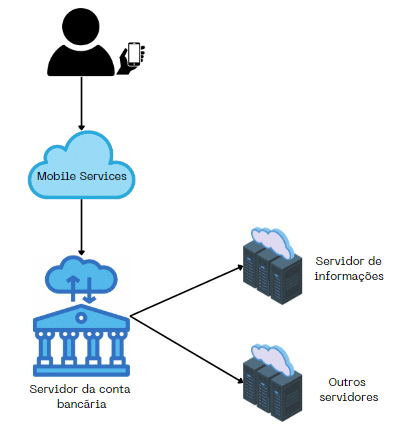
\includegraphics[width=6cm]{Imagens/arcB.png} 
    \caption{Arquitetura de uma aplicação de banco móvel}
    \label{arcB}
    \end{figure}
    
    Como proposto por \citeonline{Ahmad2015}, as aplicações bancárias móvel carregam uma arquitetura simples por conter apenas ações e validações internas da própria instituição, como pode-se ver na figura \ref{arcB}. O dispositivo utilizado, que é acessado pelo usuário para interagir com o sistema, exibi os menus e transmite mensagens curtas de forma segura. A plataforma do banco facilita a transferência de mensagens curtas para comandos bancários compatíveis. A interação entre o usuário e o provedor de serviços ocorre por meio de diálogos multiníveis, com o banco fornecendo suporte e executando instruções nas contas bancárias. O Sistema de banco móvel também suporta a comunicação com outros servidores contribuindo para a ampliação dos serviços oferecidos ao usuário.
    

    \subsection{PCI DSS}
    \label{pci}

    O Payment Card Industry Data Security Standard (PCI DSS) é um conjunto de normas de segurança criado com o objetivo de proteger os dados dos usuários de serviços de pagamento e assegurar que as empresas que processam, armazenam ou transmitem essas informações mantenham um ambiente seguro. Este padrão foi estabelecido pelo PCI Security Standards Council \cite{pci2022}, um fórum global independente formado em 2006 por grandes marcas de cartões de crédito, incluindo Visa, MasterCard, American Express, Discover e JCB, que colaboram para melhorar a segurança dos pagamentos em todo o mundo.
    
    Segundo \citeonline{Seaman2020}, e seu uso é obrigatório pelas marcas de cartão, o que a torna uma das certificações de segurança internacional mais reconhecidas do mercado de pagamentos. O método de avaliação é aplicado a qualquer empresa que processe, armazene ou transmita dados de cartões de crédito e débito, independentemente do tamanho da organização ou do volume de transações processadas. Empresas que não se adéquam às normas estão sujeitas a receberem multas e até mesmo a serem descredenciadas junto às operadoras e bandeiras de cartão de crédito.

    \subsubsection{Requisitos da certificação}
    Para estar em conformidade com o PCI DSS, todas as empresas devem atender a 12 requisitos básicos, organizados em 6 categorias abrangentes que cobrem desde a construção e manutenção de uma rede segura até a implementação de políticas robustas de segurança da informação, conforme descrito pela \citeonline{pci2022}:
    
    \begin{enumerate}
        \item Construir e manter uma rede e sistemas seguros
            \begin{enumerate}
            \item Instalar e manter controles de segurança de rede. 
            \item Aplicar as configurações de segurança para todos os componentes de sistema.
            \end{enumerate}

        \item Proteger os dados da conta
            \begin{enumerate}
            \item Proteger os dados da conta armazenados.
            \item Proteger os dados do titular do cartão com criptografia forte durante a transmissão em redes públicas abertas.
            \end{enumerate}

        \item Manter um programa de gestão de vulnerabilidade
            \begin{enumerate}
            \item Proteger todos os sistemas e redes de software malicioso.
            \item Desenvolver e manter sistemas e software seguros.
            \end{enumerate}

        \item Implementar medidas fortes de controle de acesso
            \begin{enumerate}
            \item Restringir o acesso aos componentes de sistema e aos dados do titular do cartão por necessidade de conhecimento do negócio.
            \item Identificar usuários e autenticar o acesso aos componentes de sistema
            \item Restringir o acesso físico aos dados do titular do cartão.
            \end{enumerate}

        \item Monitorar e testar as redes regularmente
            \begin{enumerate}
            \item Registrar e monitorar todo o acesso aos componentes de sistema e dados do titular do cartão.
            \item Testar a segurança de sistemas e redes regularmente.
            \end{enumerate}

        \item Manter uma política de segurança da informação
            \begin{enumerate}
            \item Apoiar a segurança da informação com políticas e programas organizacionais.
            \end{enumerate}
    \end{enumerate}

    \subsubsection{Importância do PCI DSS}
    A importância do PCI DSS vai além do simples cumprimento de uma norma de segurança; ele é um pilar fundamental para a proteção das transações financeiras em um mundo cada vez mais digitalizado. A conformidade com o PCI DSS ajuda a prevenir a exposição de informações sensíveis dos titulares de cartões, reduzindo significativamente o risco de fraudes e violações de dados. Considerando o volume de transações realizadas diariamente, uma falha de segurança pode ter consequências catastróficas, tanto financeiras quanto reputacionais, para as empresas envolvidas.

    A conformidade com o PCI DSS também facilita a criação de um ambiente de segurança robusto dentro da organização. Ao seguir as diretrizes estabelecidas pelo padrão, as empresas desenvolvem uma cultura de segurança da informação que permeia toda a sua estrutura. Isso não só protege os dados dos titulares de cartões, mas também fortalece as defesas contra outros tipos de ameaças cibernéticas, como ataques de malware e violações internas. A implementação contínua dessas práticas de segurança ajuda a garantir que as empresas estejam melhor preparadas para enfrentar novos desafios no cenário de cibersegurança.

    No contexto regulatório, o PCI DSS serve como uma base para o cumprimento de outras normativas e leis de proteção de dados, como o General Data Protection Regulation (GDPR) na Europa e a Lei Geral de Proteção de Dados (LGPD) no Brasil. Embora o PCI DSS seja específico para o setor de pagamentos, sua implementação pode ser um passo inicial para a conformidade com esses outros regulamentos, criando uma sinergia entre as diferentes exigências legais.
    
    \section{Engenharia de Requisitos}
    Segundo \citeonline{Pohl2015}, os requisitos de um sistema são descrições das funcionalidades que o sistema deve possuir, os serviços que ele oferece e condições ou capacidades que deve ser atendida ou possuídas pelo mesmo. Esses requisitos refletem as necessidades dos clientes para um sistema que atende a uma finalidade específica,  quais são suas demandas e dores e o que é necessário para solucioná-la, dentro do que está sendo proposto. O processo de descobrir, analisar, documentar e verificar esses serviços e restrições é conhecido como engenharia de requisitos. 
    
    Os requisitos de software são frequentemente classificados como requisitos funcionais e requisitos não funcionais:
    
    \subsection{Requisitos funcionais}
    Os requisitos funcionais de um sistema descrevem as funcionalidades que ele deve executar. Esses requisitos variam conforme o tipo de software a ser desenvolvido, seus possíveis usuários e a abordagem adotada pela organização ao redigir os requisitos. Quando expressos como requisitos de usuário, são normalmente descritos de maneira abstrata, para garantir a compreensão pelos usuários do sistema. No entanto, requisitos funcionais de sistema mais específicos detalham as funções do sistema, suas entradas e saídas, e as exceções. Esses requisitos podem variar de descrições gerais, que abrangem as principais funcionalidades do sistema, até especificações muito detalhadas, que refletem as operações e processos específicos de uma organização.
    
    \subsection{Requisitos não funcionais}
    Os requisitos não funcionais são aqueles que não estão diretamente ligados aos serviços específicos que o sistema oferece aos seus usuários. Eles se relacionam às propriedades emergentes do sistema, como confiabilidade, tempo de resposta e uso de recursos. Esses requisitos normalmente especificam ou restringem as características do sistema como um todo, como mostrado na figura \ref{naofunc}, o que os torna frequentemente mais críticos que requisitos funcionais individuais.
    
    
    \subsubsection{Requisitos de segurança}
    De acordo com \citeonline{Dalpiaz2016}, requisitos de segurança constituem um conjunto de diretrizes, normas e práticas essenciais para assegurar a proteção de um sistema ou ambiente. Esses requisitos são desenvolvidos a partir de análises de risco detalhadas, levando em conta as possíveis ameaças que poderiam comprometer a segurança dos ativos de uma organização e podem ser classificados em várias categorias principais, como autenticação, autorização, confidencialidade, integridade, disponibilidade, conscientização e treinamento, cada um com seu papel e importância na implementação e uso seguro de sistemas de informação.

    \begin{figure}[H]
    \centering 
    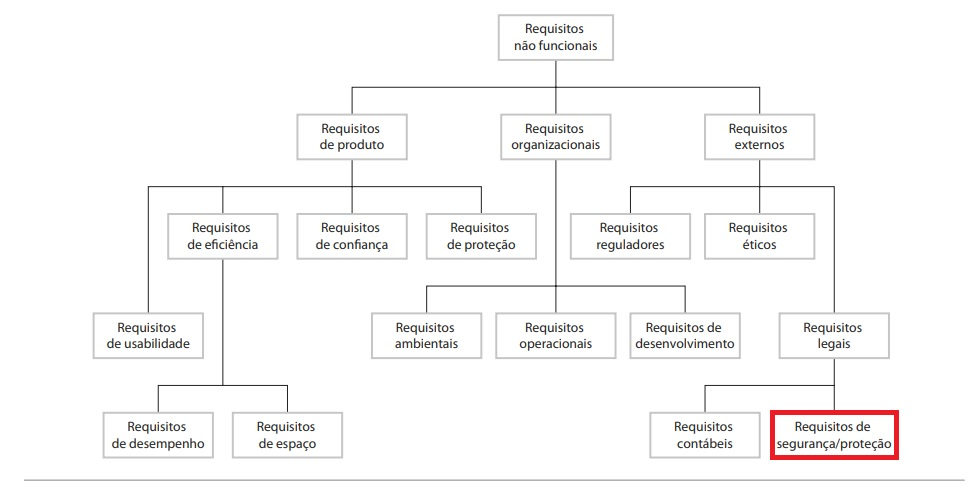
\includegraphics[width = 16cm]{Imagens/naofucnionais.jpg}
    \caption{Tipos de requisitos não funcionais}
    \cite{sommerville2011}
    \label{naofunc}
    \end{figure}
    
    Definir requisitos de segurança eficazes pode ser desafiador devido à complexidade dos sistemas modernos e à diversidade das ameaças, como vemos na seção  \ref{owasp}. Requisitos de segurança devem ser claros, mensuráveis e verificáveis. Eles também precisam ser adaptáveis para evoluir com as novas ameaças e tecnologias emergentes.
    
    
    \subsection{Ciclo de vida da Engenharia de requisitos}
    
    A Engenharia de Requisitos envolve várias fases que se repetem em um ciclo contínuo: Estudo de Viabilidade, Elicitação, Modelagem e Análise, Validação e Gerenciamento. Durante o desenvolvimento e a manutenção do software, essas etapas são continuamente realizadas para analisar os problemas e as necessidades do projeto, oferecendo soluções baseadas nos requisitos definidos. Esse ciclo é baseado nas atividades definidas e descritas por \citeonline{sommerville2011}.
    
    \subsubsection{Estudo de Viabilidade}
    O ciclo de vida da engenharia de requisitos começa com o Estudo de Viabilidade, uma fase crucial para determinar a viabilidade técnica, econômica e operacional do projeto. Nesta etapa, os analistas de sistemas realizam uma série de investigações para avaliar se os requisitos iniciais podem ser satisfeitos dentro das restrições de recursos, tempo e tecnologia disponíveis. É uma análise abrangente que busca responder a perguntas fundamentais como: "É tecnicamente possível desenvolver este sistema?", "Os benefícios superam os custos?", e "A organização está preparada para adotar essa solução?". Esta fase também envolve a identificação de possíveis riscos e a definição de estratégias para mitigá-los, ajudando a decidir se o projeto deve avançar, ser modificado ou mesmo abandonado.
    
    \subsubsection{Elicitação}
    Após a viabilidade do projeto ser confirmada, inicia-se a etapa de Elicitação de Requisitos, onde se busca compreender as necessidades e expectativas dos usuários e das partes interessadas. Esta fase é fundamental para garantir que os requisitos coletados sejam completos e representativos das verdadeiras necessidades do negócio. Diversas técnicas são empregadas para coletar essas informações, incluindo entrevistas, questionários, workshops, observações diretas, e análise de documentos existentes. A elicitação é um processo interativo que exige comunicação eficaz e colaboração entre os analistas de sistemas e os stakeholders. O objetivo é assegurar que todos os requisitos relevantes sejam identificados e compreendidos.
    
    \subsubsection{Modelagem e Análise}
    Com os requisitos coletados, a próxima etapa é a Modelagem e Análise. Nesta fase, os requisitos são organizados e representados de maneira estruturada, utilizando ferramentas de modelagem como diagramas de casos de uso, diagramas de atividades e modelagem de processos. Estas representações visuais ajudam a clarificar os requisitos, identificar lacunas, redundâncias e possíveis conflitos. A análise dos requisitos também envolve a verificação de sua completude, consistência e viabilidade. É nesta fase que os requisitos são refinados e detalhados, assegurando que estejam claros e compreensíveis tanto para a equipe técnica quanto para os stakeholders.
    
    \subsubsection{Validação}
    Uma vez modelados e analisados, os requisitos devem ser validados. A Validação é a etapa onde se verifica se os requisitos realmente refletem as necessidades e expectativas dos usuários e se são viáveis do ponto de vista técnico. Esta fase pode envolver revisões de requisitos, prototipagem, simulações e testes de requisitos para garantir que os requisitos são corretos e completos. A validação é um processo colaborativo que envolve revisões com as partes interessadas para confirmar que o sistema desenvolvido atenderá às suas expectativas e requisitos. O objetivo é garantir a qualidade e a aderência dos requisitos às necessidades reais do projeto.
    
    \subsubsection{Gerenciamento}
    Por fim, a etapa de Gerenciamento de Requisitos é um processo contínuo que se estende por todo o ciclo de vida do projeto. O gerenciamento de requisitos envolve a rastreabilidade, controle de versões e controle de mudanças nos requisitos. Ferramentas e técnicas de gerenciamento são utilizadas para manter a documentação atualizada, avaliar o impacto de alterações nos requisitos e comunicar essas mudanças às partes interessadas. Esta etapa é crucial para manter a integridade e consistência dos requisitos ao longo do desenvolvimento do sistema, garantindo que todas as mudanças sejam aprovadas e documentadas adequadamente.
    
    
    \subsection{Importância da engenharia de requisitos na segurança}

    A engenharia de requisitos desempenha um papel fundamental na segurança da informação, pois estabelece as bases sobre as quais sistemas seguros são construídos. Segundo  \citeonline{Dalpiaz2016}, a definição precisa e clara dos requisitos de segurança é essencial para antecipar e mitigar possíveis ameaças e vulnerabilidades que possam comprometer a integridade, confidencialidade e disponibilidade dos dados. Sem uma sólida engenharia de requisitos, os sistemas correm o risco de apresentar brechas que podem ser exploradas por agentes maliciosos, resultando em perdas financeiras, danos à reputação e outras consequências graves.

    Um dos principais aspectos da engenharia de requisitos na segurança da informação é a capacidade de identificar e entender as ameaças e riscos específicos ao contexto do sistema em desenvolvimento. Ao envolver todas as partes interessadas, incluindo analistas de segurança, desenvolvedores, e usuários finais, a engenharia de requisitos garante que todas as perspectivas sejam consideradas. Este processo colaborativo é crucial para a identificação de possíveis pontos fracos e para a definição de medidas de segurança que sejam práticas e eficazes no contexto operacional real do sistema.
    
    A engenharia de requisitos também é vital para a integração de segurança ao longo de todo o ciclo de vida do desenvolvimento de software. Ao definir claramente os requisitos de segurança desde as fases iniciais, é possível incorporar práticas de segurança em cada etapa do desenvolvimento, desde o design até a implementação e testes. Isso não só aumenta a robustez do sistema contra ataques, mas também reduz os custos associados à correção de falhas de segurança descobertas em estágios mais avançados, onde tais correções são tipicamente mais dispendiosas e complexas.
    
    Além disso, a documentação precisa e detalhada dos requisitos de segurança facilita a comunicação e o entendimento entre todos os membros da equipe de desenvolvimento. Ela serve como uma referência clara para desenvolvedores, testadores e auditores, garantindo que todos estejam cientes das exigências de segurança e das justificativas por trás de cada medida implementada. Isso promove uma cultura de segurança dentro da organização, onde a proteção dos dados é vista como uma responsabilidade compartilhada.
    

    \section{Modelos e padrões de segurança para aplicações móveis}
    As aplicações móveis enfrentam diversas ameaças de segurança, sendo essencial a adoção de diretrizes robustos para mitigar esses riscos. Estes modelos e padrões são fundamentais para o desenvolvimento de aplicações móveis seguras, oferecendo diretrizes claras e práticas recomendadas para enfrentar os desafios de segurança específicos deste ambiente. Ao aderir a estes padrões, desenvolvedores e organizações podem melhorar significativamente a segurança de suas aplicações móveis, protegendo os dados dos usuários e garantindo a integridade e a confiabilidade dos serviços oferecidos.

    \subsection{OWASP MASVS}
    O OWASP Mobile Application Security Verification Standard (MASVS) \cite{masvs2019} é um padrão globalmente reconhecido para a segurança de aplicações móveis. Ele fornece um conjunto de requisitos de segurança que podem ser utilizados como base para avaliar a segurança de uma aplicação móvel. O MASVS é dividido em várias categorias, incluindo arquitetura de segurança, manipulação de dados, autenticação, gerenciamento de sessão, criptografia e comunicação. Cada categoria contém requisitos específicos que devem ser atendidos para garantir a segurança da aplicação. O objetivo do MASVS é ajudar desenvolvedores, testadores de segurança e arquitetos a garantir que as aplicações móveis sejam desenvolvidas e testadas de acordo com as melhores práticas de segurança.
    
    \subsection{NIST SP 800-163}
    O NIST Special Publication 800-163 \cite{Ogata2019} fornece diretrizes detalhadas para a avaliação da segurança de aplicações móveis. Este documento aborda o processo de verificação de segurança, incluindo a identificação de ameaças e vulnerabilidades, avaliação de riscos e implementação de controles de segurança. O NIST SP 800-163 destaca a importância de um processo contínuo de avaliação, recomendando práticas como análises estáticas e dinâmicas de código, testes de penetração e revisões de segurança de terceiros. Este padrão é amplamente utilizado por organizações governamentais e privadas nos Estados Unidos para garantir que as aplicações móveis estejam protegidas contra ameaças emergentes.

    \subsection{ISO/IEC 27034} 
    A ISO/IEC 27034 \cite{iso2018} é um padrão internacional que aborda a segurança de aplicações, incluindo aplicações móveis, no contexto do ciclo de vida do desenvolvimento de software. Este padrão fornece um framework abrangente para integrar práticas de segurança em todas as fases do desenvolvimento, desde o planejamento até a implementação e manutenção. A ISO/IEC 27034 enfatiza a importância de uma abordagem baseada em riscos, onde a segurança é adaptada às necessidades específicas da aplicação e do ambiente operacional. Além disso, o padrão define um conjunto de controles de segurança que podem ser aplicados para mitigar riscos específicos, promovendo a criação de aplicações mais seguras e resilientes.